\documentclass[10pt]{beamer}
\usepackage{xeCJK}
\usepackage{graphicx}
\usepackage{booktabs}
\usepackage{listings}
\usepackage{multirow}
\usepackage{mathtools}
\usepackage{ulem}
\usetheme{metropolis}
\begin{document}
\title{水题讨论}
\date{\today}
\author{huhao}
\maketitle
\clearpage
\begin{frame}
	\frametitle{1.1 AGC040F Two Pieces}

	你有两个棋子,若某时刻棋子位置为:$(a,b)$($a\le b$),那么你可以让它们位置变为:$(b,b),(a+1,b),(a,b+1)$。

	问$t$时刻后棋子位置为$(x,y)$的方案。

	两方案不同当且仅当某时刻棋子位置不同,棋子不作区分,即,$(x,y)$和$(y,x)$认为是相同的。

	$1\le t\le 10^7,0\le x\le y\le t$

	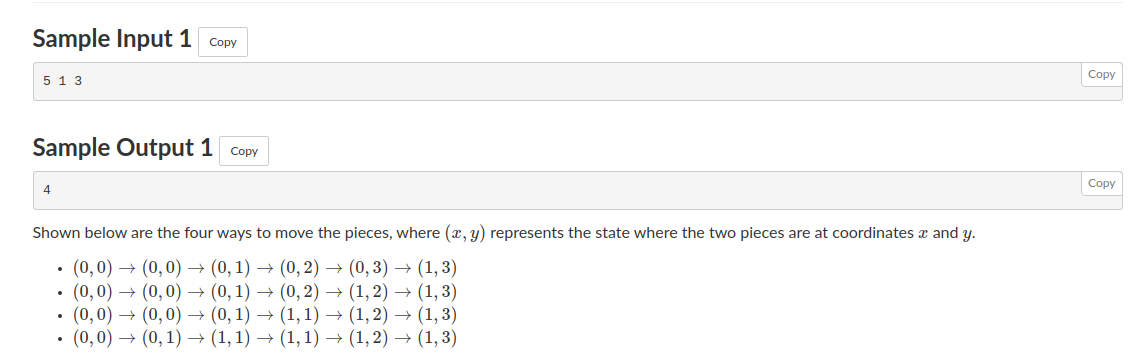
\includegraphics[width=0.9\textwidth]{1.png}

\end{frame}
\clearpage
\begin{frame}
	\frametitle{1.2 AGC040F solution}

	\onslide<1-> 记状态$(a,b)$表示位置$(a,a-b)$,那么每一次可以变为:$(a+1,b+1),(a,b-1),(a,0)$

	\onslide<1-> 为了去重,第二个操作要求$b\ge 2$

	\onslide<2-> 于是我们可以记一个由$\{1,2,3\}$组成的操作序列,表示第$i$次的操作

	\onslide<2-> 那么操作序列长为$t$,且$1$出现$y$次

	\onslide<3-> 于是可以只考虑$b$的值,考虑枚举$3$出现次数$t_0$

	\onslide<4-> 若$t_0=0$,则是一个经典的格路计数题:求由$(0,0)$走到$(t-y,y-x)$,每一次可以走向量$(1,-1)$或$(1,1)$,不经过$y=0,x>0$的方案数

	\onslide<5-> 考虑推广,不考虑$3$的话会是一个到$(t,y-(t-y-t_0))$的路径,只要在纵坐标为$y-(t-y-t_0)-(y-x)$时执行一次$3$操作即可

	\onslide<6-> 另外如果一个位置可以插入$3$当且仅当后面的纵坐标都比它大,所以转化为:一共$y-(t-y-t_0)-(y-x)+1$个位置,且最后一个必须放,前面的可放可不放,问方案数

\end{frame}
\clearpage
\begin{frame}
	\frametitle{Epilogue}

	\begin{center}
		\Huge Thanks for listening!
	\end{center}

\end{frame}
\end{document}